\documentclass[prb,twocolumn]{revtex4-2}
\usepackage{graphicx}
\usepackage{amsmath}
\usepackage{amssymb}
\usepackage{float}
\usepackage{epstopdf}

\begin{document}
\title{Assignment 6}

\author{James Lawton}
\affiliation {
Physics Department, Virginia Tech, Blacksburg, Virginia 24061, USA\\
}


\begin{abstract}
Abstract: Using the Relaxation, Crank-Nicholson, Euler, and Monte Carlo Methods
    in order to solve different equations.
\end{abstract}

\maketitle

\section{Problem 1}

\noindent

Here the Relaxation method is used to plot the potential of the Poisson
equation: 

\begin{eqnarray}
\nabla^2 \phi(x, y) = -\rho(x, y)/\epsilon_0
\end{eqnarray}

for the following two sets of conditions:

(a)

$\rho(x, y) = 0$,

$\phi(0, y) = \phi(L_x, y) = \phi(x, 0) = 0$,

$\phi(x, L_y) = 1 V, L_x = 1 m$,

$L_y = 1.5 m$
\label{Poisson Conditions a}

(b)

$\rho(x, y)/\epsilon_0 = 1 V/m^2$,

$\phi(0, y) = \phi(L_x , y) = \phi(x, 0) = \phi(x, L_y ) = 0$,

$L_x = L_y = 1 m$

Then each scenario is plotted in 3D with these two starting conditions:

(a)

\begin{figure}[H]
    \centerline{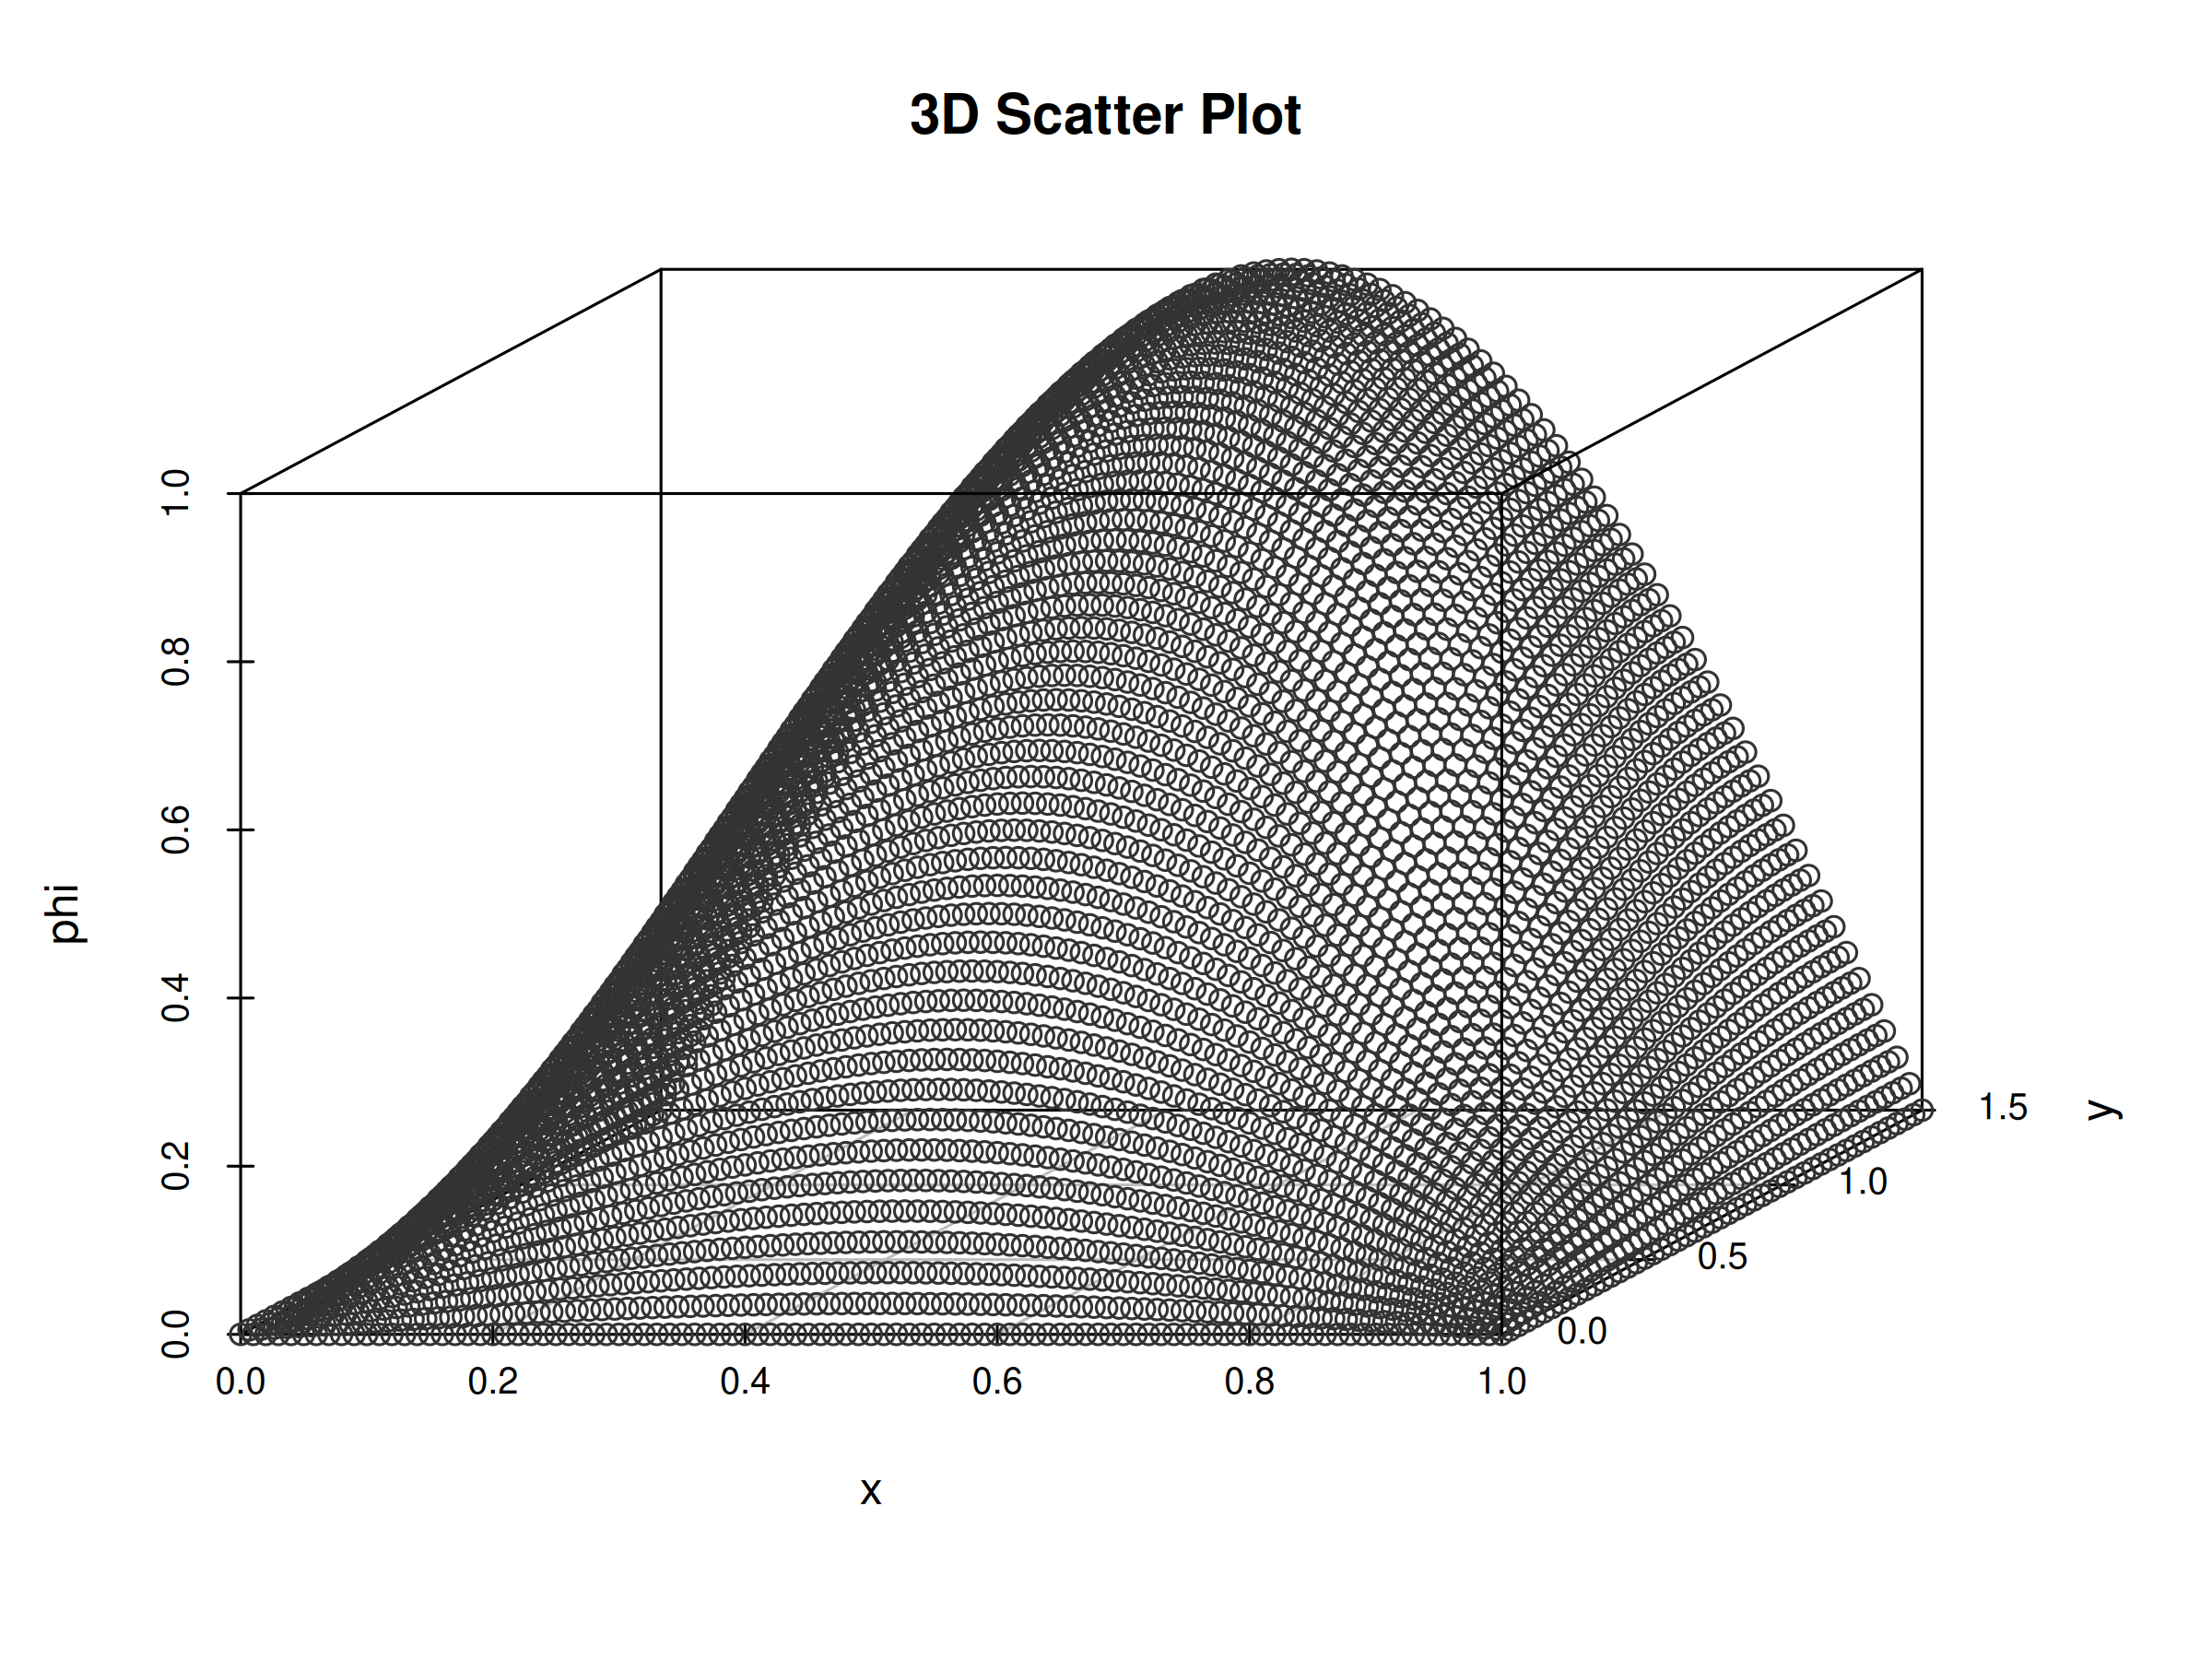
\includegraphics [width=3 in] {p1/p1a_init.png}}
    \caption{Condition (a) Initial} \label{q1}
\end{figure}

(b)

\begin{figure}[H]
    \centerline{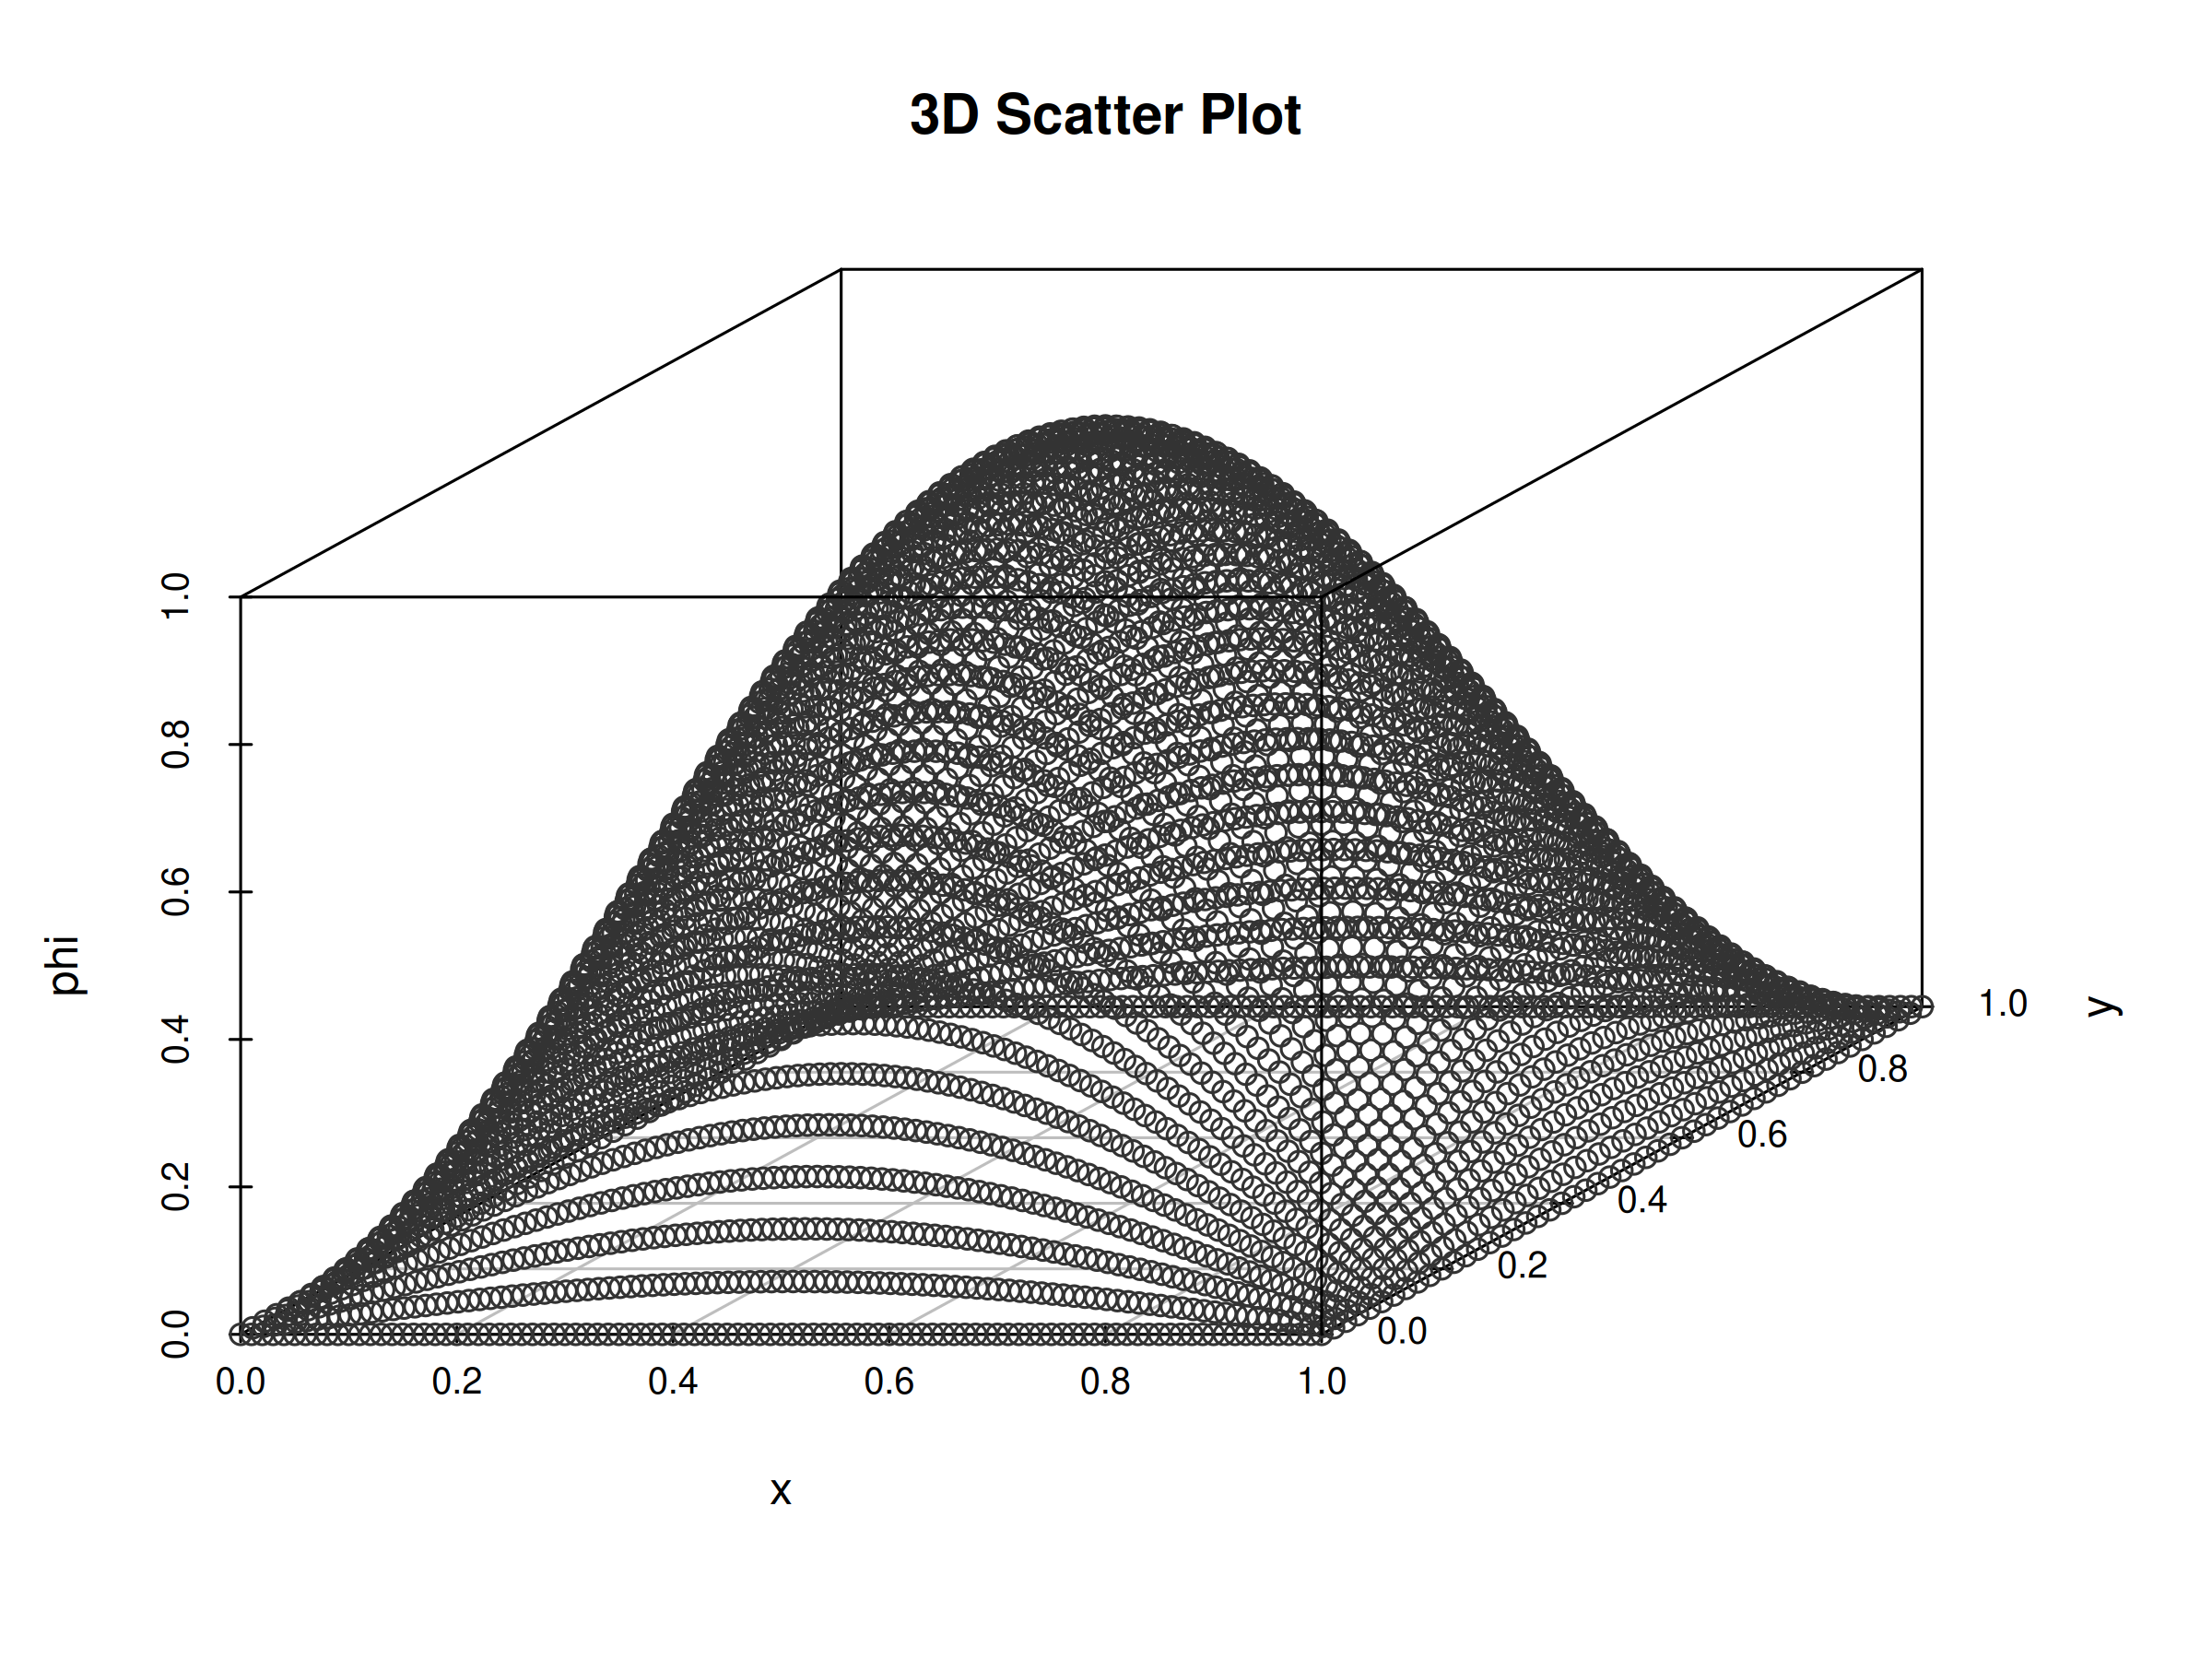
\includegraphics [width=3 in] {p1/p1b_init.png}}
    \caption{Condition (b) Initial} \label{q1}
\end{figure}

After running the algorithm we get the following results

(a)

\begin{figure}[H]
    \centerline{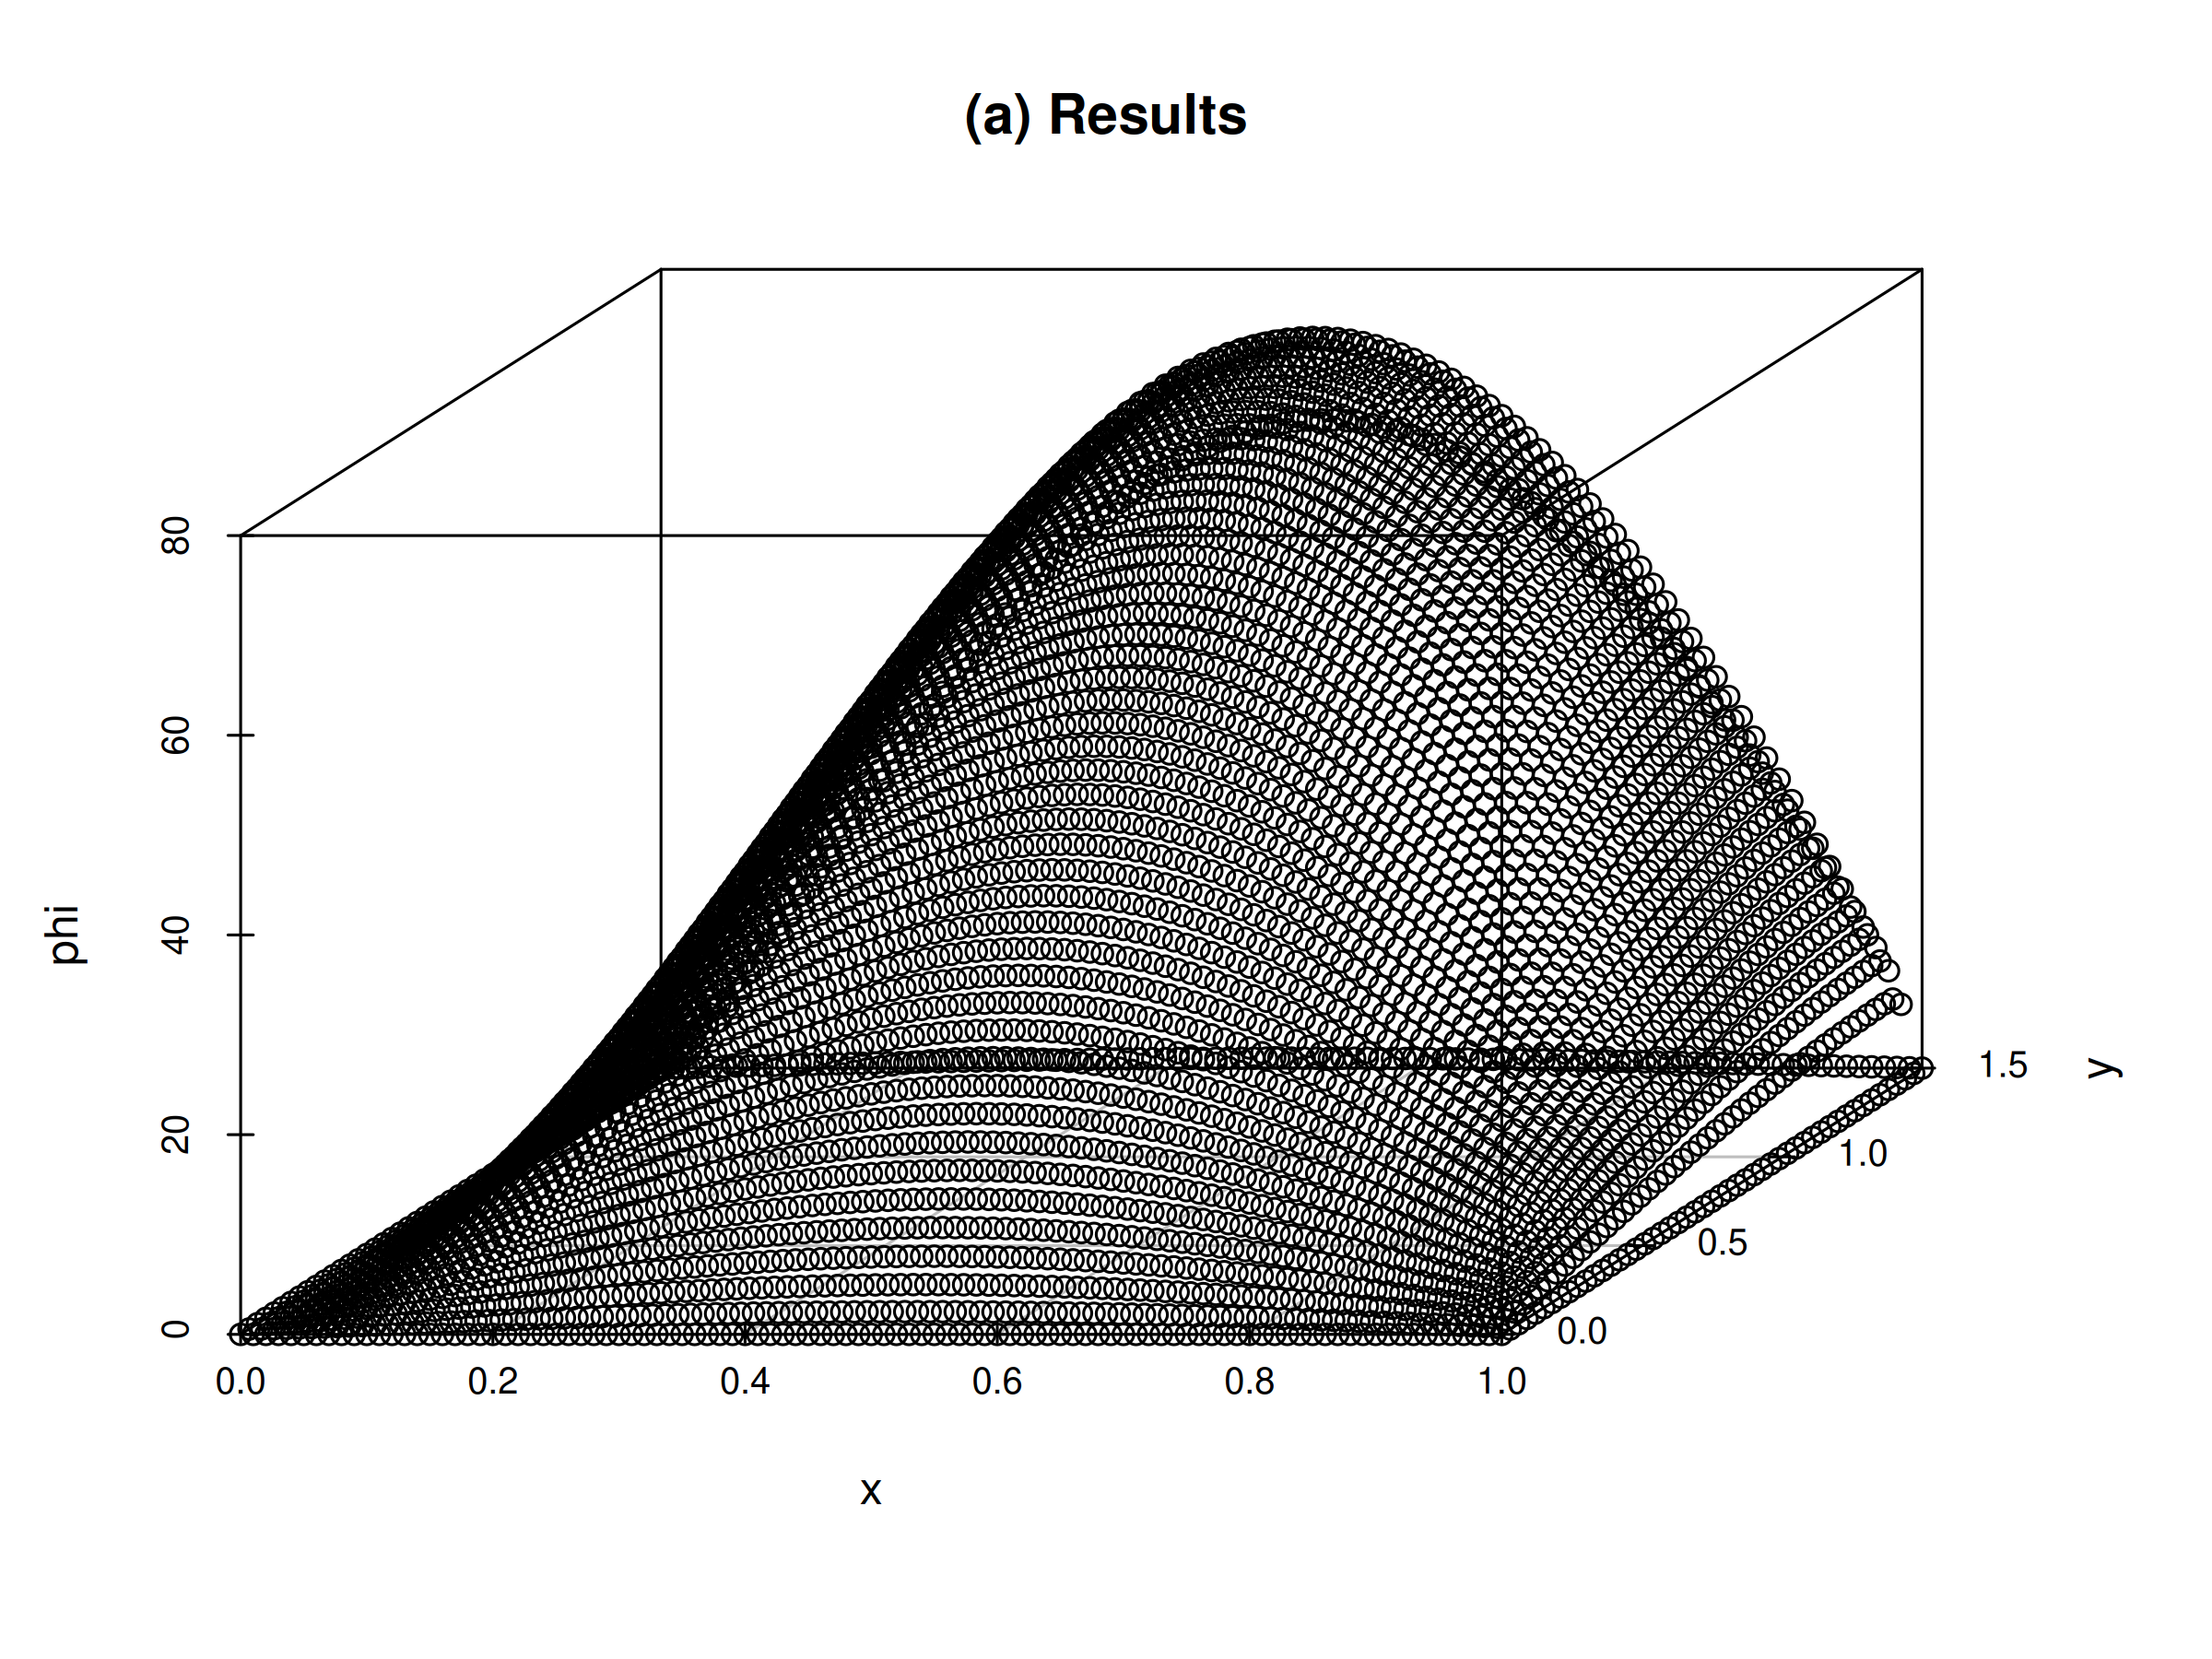
\includegraphics [width=3 in] {p1/p1a}}
    \caption{Condition (a) Results} \label{q1}
\end{figure}

(b)

\begin{figure}[H]
    \centerline{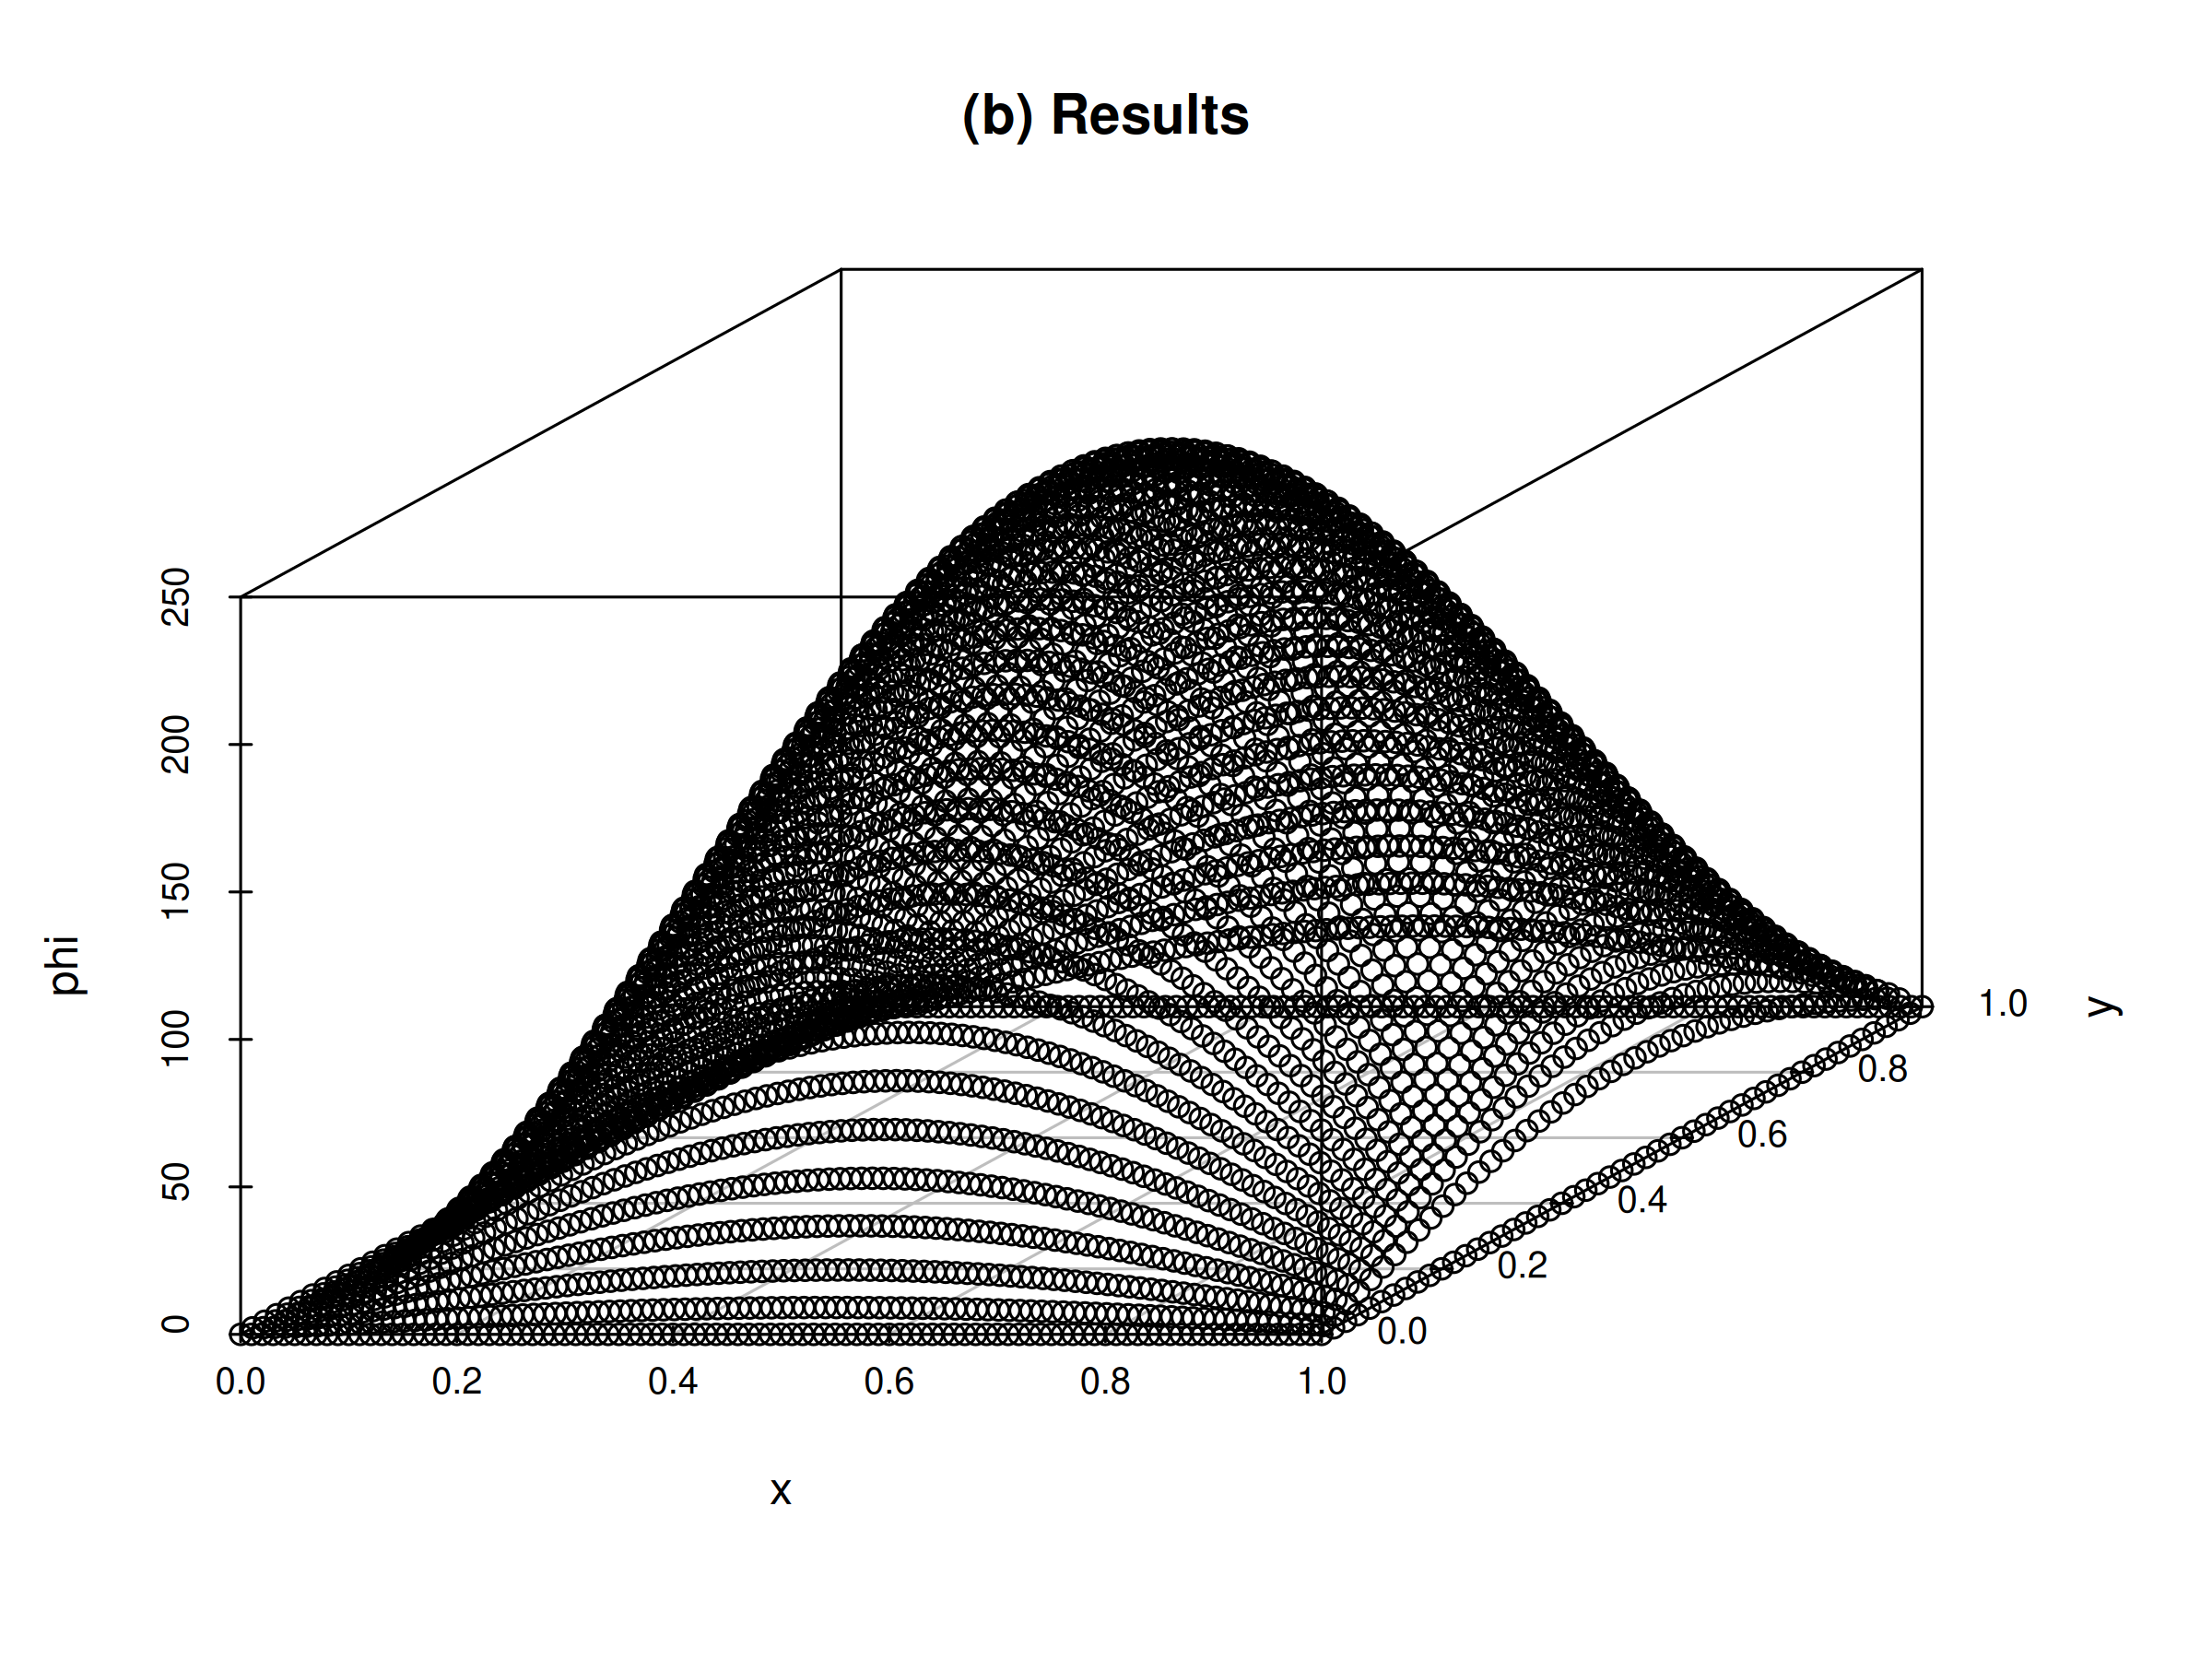
\includegraphics [width=3 in] {p1/p1b}}
    \caption{Condition (b) Results} \label{q1}
\end{figure}

We can see that in both scenarios the amplitude of the plot grew, with the plot
(a) growing to a peak of ~80 with a sharp drop back to zero, and plot (b)
growing to a peak of 250 with relatively similar proportions.

\section{Problem 2}

Here we look to model a diffusion equation for a rod of nuclear waste as
depicted in the diagram below:

\begin{figure}[H]
    \centerline{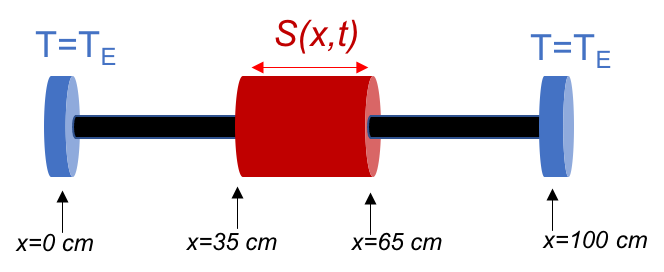
\includegraphics [width=3 in] {p2/plot_rod.png}}
    \caption{Nuclear waste diagram} \label{q1}
\end{figure}

The following equation models the temperature diffusion across the horizontal
axis:

\begin{eqnarray}
    \frac{1}{\kappa}
    \frac{\partial T(x,t)}{\partial t} -
    \frac{\partial^2 T(x,t)}{\partial^x x} =
    S(x,t)
\end{eqnarray}

The following boundary conditions will be used reflecting the diagram:

$S(x,t) = \frac{T_0}{a^2}e^{-t/\tau_0}$,
for $x > 35$cm, and $x < 65$cm, but $S(x,t)=0$ otherwise

\subsection{The Crank-Nicholson Method}

Here is the solution having used the Crank-Nicholson method using the distance
across rather than the distance from the center:

\begin{figure}[H]
    \centerline{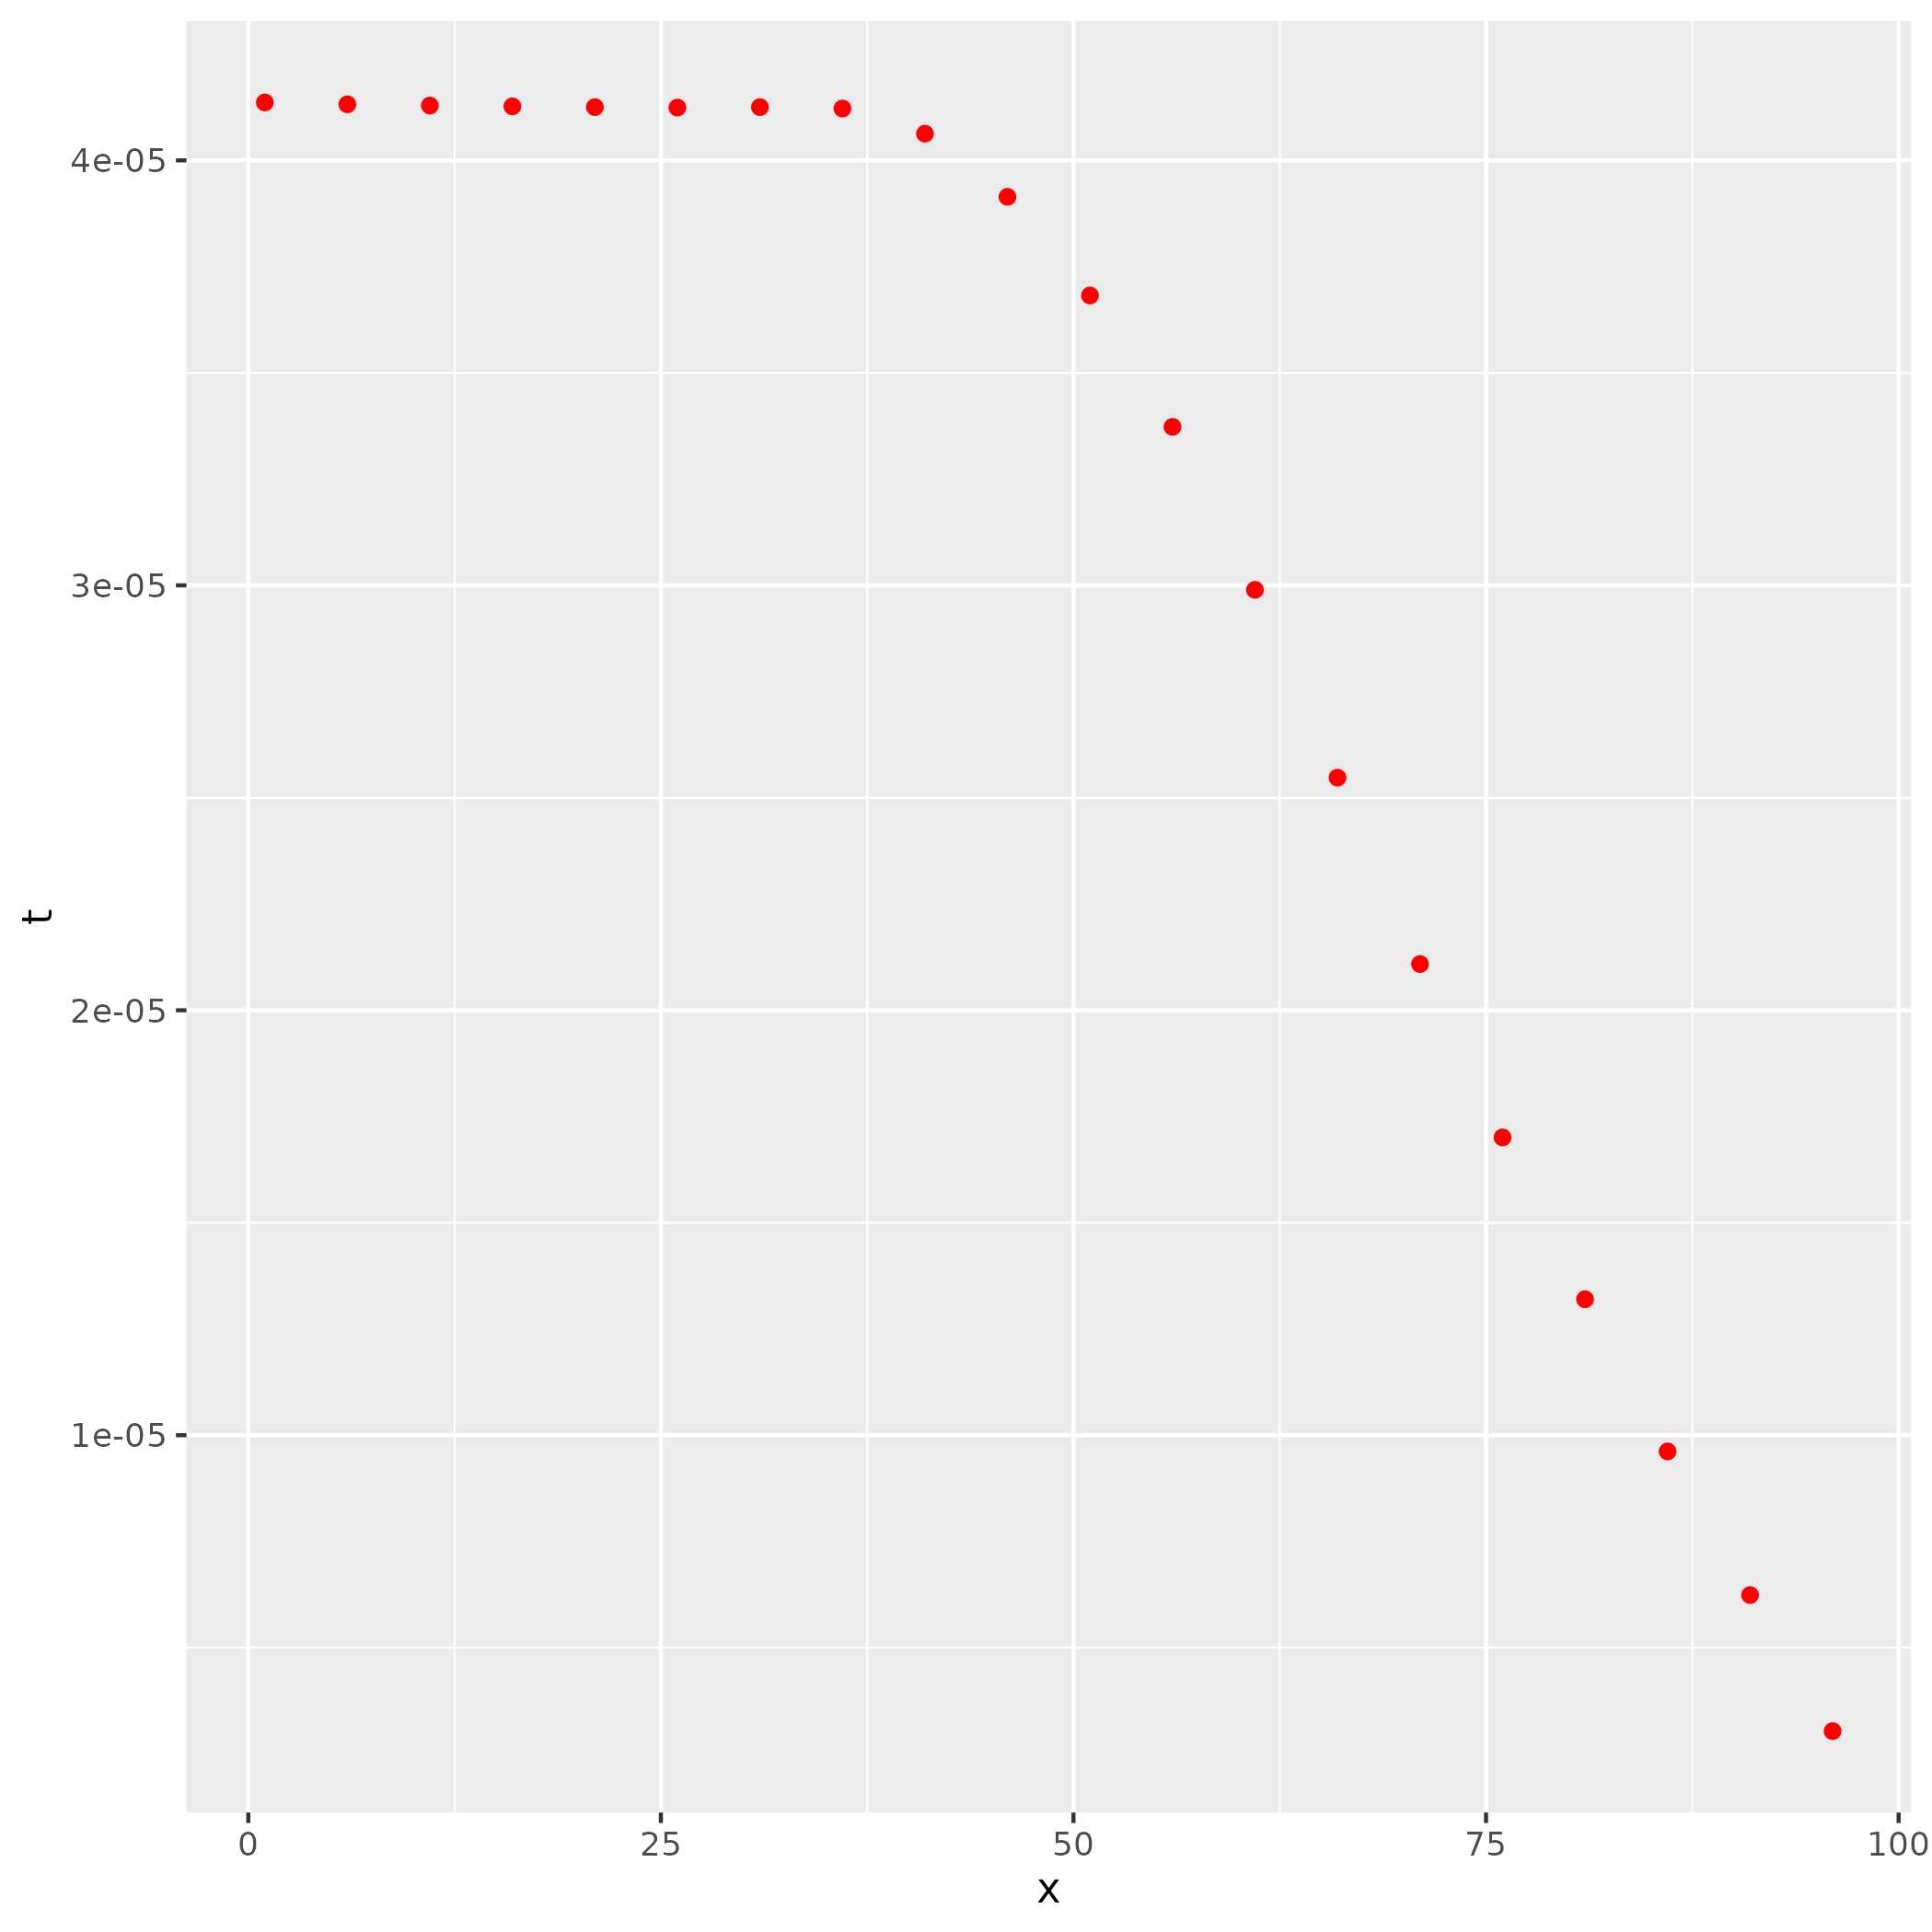
\includegraphics [width=3 in] {p2/crank}}
    \caption{Temperature of nuclear rod across x} \label{q1}
\end{figure}

We can see that this is not the expected output as it should be symmetrical
across $x=50$ with both ends tapering off towards zero. This graph still looks 
like it's measuring the temperature relative to the radius similar to a bell 
curve. The modifications made to the java file were not effective enough in
changing it to plot the x rather than the radius.

Another unexpected result is the very small values obtained with all the values
being within the magnitude of $4.5*10^{-5}$

% \subsection{The Euler Method}

\section{Problem 3}

We will calculate the following integral using the Monte-Carlo Method using the
Metropolis Algorithm:

\begin{eqnarray}
    S = \int_{-\infty}^{\infty} e^{-r^2/2} (xyz)^2 dr
\end{eqnarray}

Here are the solutions to the integral plotted over the number of Monte-Carlo
steps:

\begin{figure}[H]
    \centerline{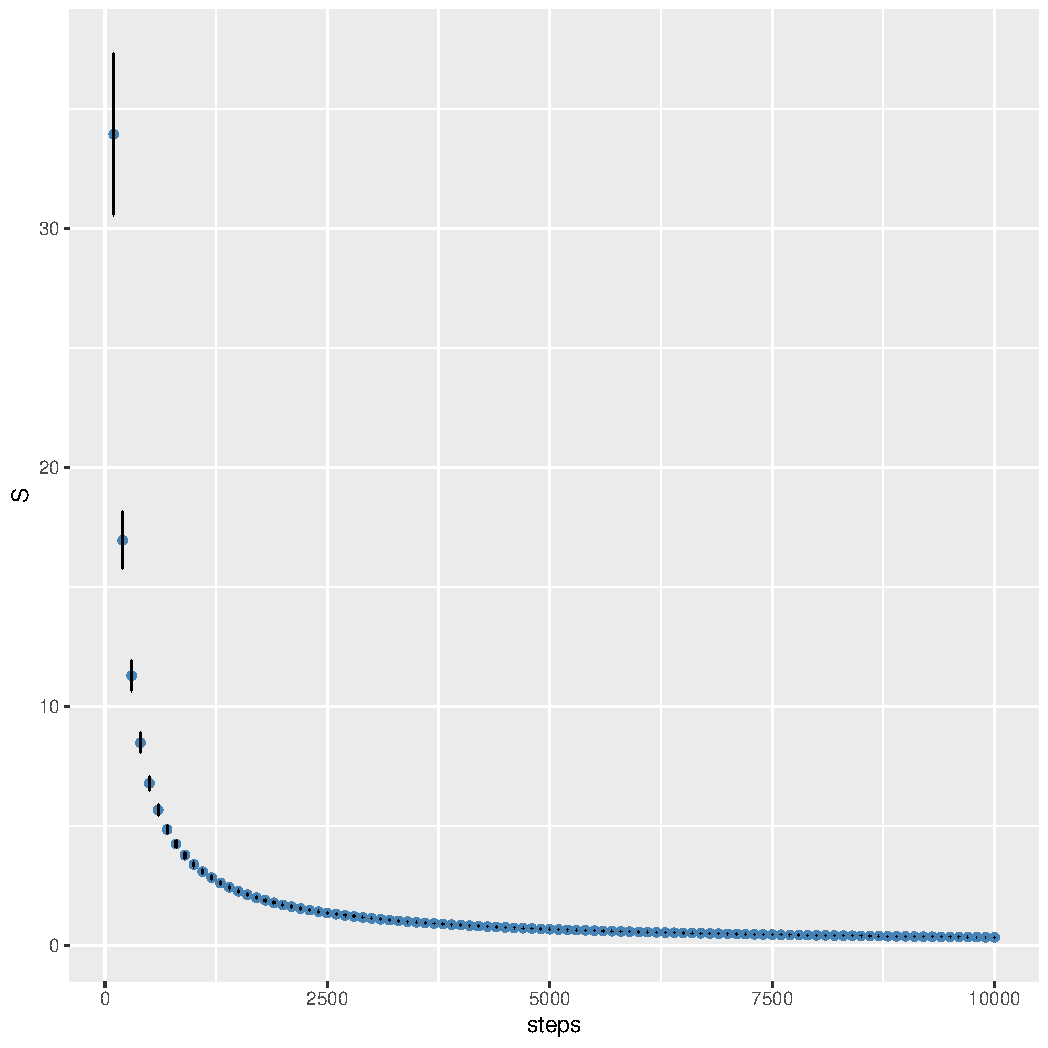
\includegraphics [width=3 in] {p3/p3}}
    \caption{Integral solved by Monte-Carlo plotted against number of steps}
    \label{q1}
\end{figure}

We can observe that as the number of steps increases, the integral approaches a
single value, presumably the correct solution. The error bars also get closer
and closer to zero becoming nearly invisible early on.

\begin{thebibliography}{99}

\bibitem{thecoursetext} T. Pang, \emph{Introduction to Computational Physics},
    Cambridge University Press (2006).

\end{thebibliography}

\end{document}
